% !TEX encoding = UTF-8
% !TEX TS-program = pdflatex
% !TEX root = ../tesi.tex

%**************************************************************
\chapter{Metodi di risoluzione}
\label{cap:algoritmi}
%**************************************************************

\section{DFS}
\subsection{Descrizione}
Il primo algoritmo utilizzato per risolvere il nostro problema è stato il Depth First Search. È una strategia di ricerca non informata in quanto non si utilizzano informazioni aggiuntive sugli stati oltre alla definizione iniziale del problema.
Quindi l'algoritmo è solamente in grado di generare successori e distinguere se sono uno stato obiettivo o meno. \\
Questa strategia esplora tutti gli stati dell'albero di ricerca in profondità, cioè espande prima lo stato più profondo non ancora esplorato, ritornando indietro nel caso il cammino non porti a nessuno stato obiettivo in un numero finito di azioni. \\
Questo tipo di ricerca termina non appena trova il primo stato obiettivo, generando però, nel caso pessimo, una complessità temporale (numero di stati generati) di $\mathcal{O}(b^m)$ dove m è la massima lunghezza di un percorso e b il massimo numero di successori di uno stato, rendendo questo algoritmo poco efficiente.
\begin{figure}[h]
	\centering
	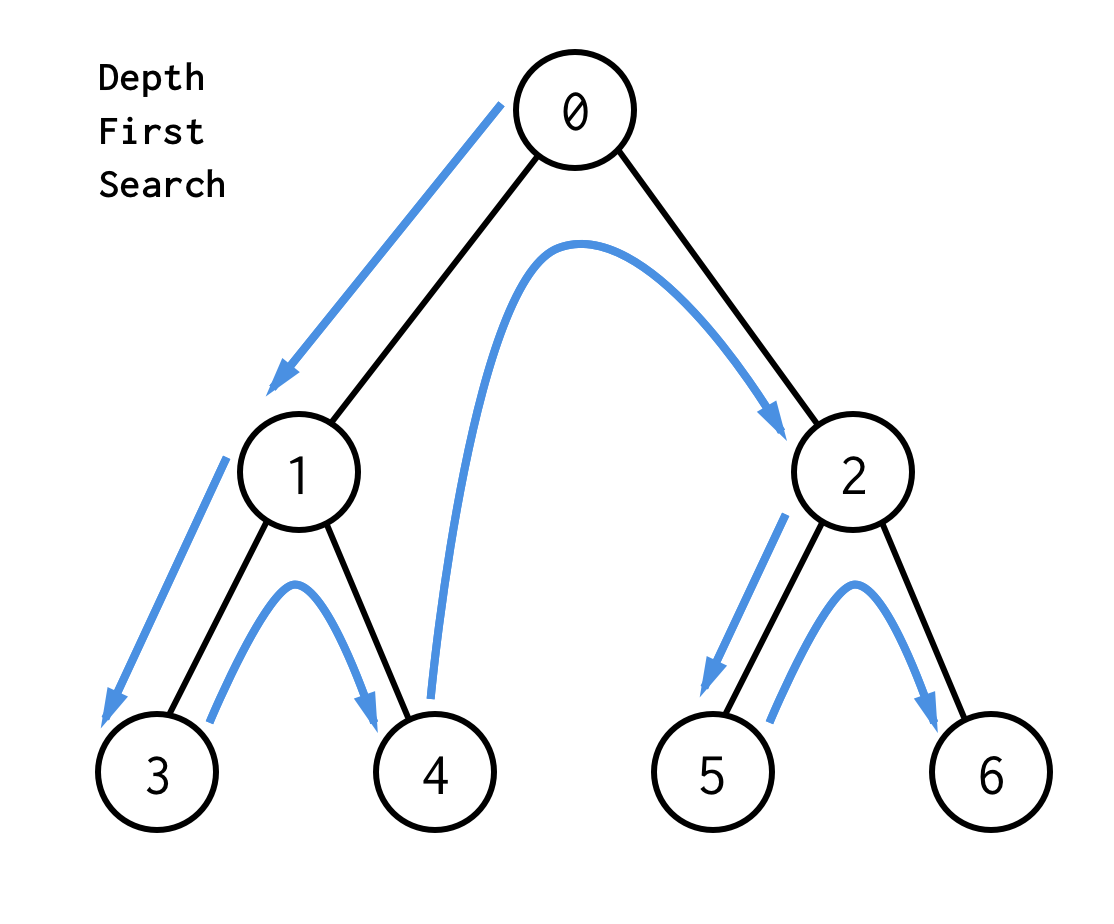
\includegraphics[scale=0.25]{immagini/dfs}
	\caption{Esempio di ricerca DFS}
	\label{fig:dfs}
\end{figure}

\subsection{Utilizzo}
Nel nostro caso l'algoritmo DFS è stato implementato in maniera ricorsiva, dove ogni stato rappresenta la configurazione attuale della griglia, intesa come forme già inserite e la loro posizione (coordinate all'interno della griglia). La configurazione iniziale della griglia rappresenta lo stato iniziale dal quale iniziale la ricerca in profondità.\\
I successori di ogni stato sono tutti i possibili posizionamenti, consistenti con l'assegnamento corrente (forme inserite e relativa posizione nella griglia), delle forme non ancora presenti nella griglia di gioco. Quindi l'algoritmo ad ogni passo sceglie la prossima forma da inserire, assegnandole il primo valore consistente nel suo dominio.
Qualora non ce ne fossero si ritorna allo stato precedente, espandendo un altro successore, fino ad arrivare ad uno stato obiettivo dove tutte le forme sono piazzate all'interno della griglia, in modo da riempirla totalmente.  \\
Essendo il nostro spazio di ricerca finito, l'algoritmo DFS ci assicura di ritornare sempre una soluzione al problema.
\begin{figure}[h]
	\centering
	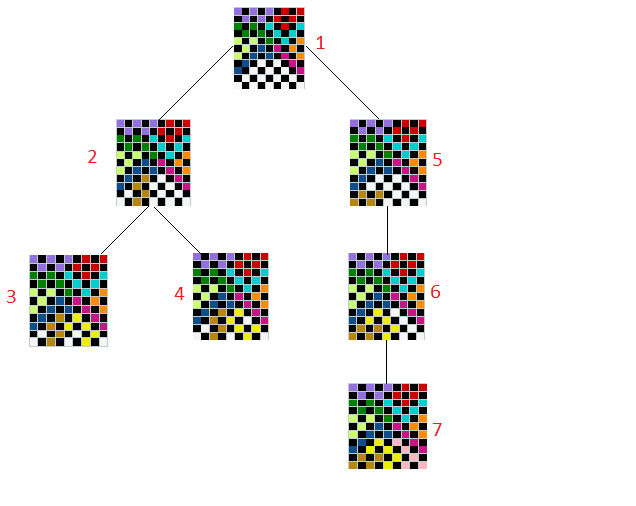
\includegraphics[scale=1]{immagini/0}
	\caption{Esempio di funzionamento dell'algoritmo DFS}
	\label{fig:0}
\end{figure}

\section{CSP}
\subsection{Descrizione}
Il secondo approccio utilizzato per risolvere questo gioco è stato formalizzare il problema in forma di CSP (Constraint Satisfaction Problem). Un CSP è composto da un insieme di variabili $X = \{X\textsubscript{1},...,X\textsubscript{n}\}$, i loro domini  $D = \{D\textsubscript{1},...,D\textsubscript{n}\}$ e un insieme di vincoli  $C = \{C\textsubscript{1},...,C\textsubscript{m}\}$, dove ogni vincolo coinvoge un sottoinsieme di variabili, specificandone una combinazione di valori permessi.\\
Uno stato è rappresentato da un assegnamento di valori ad alcune delle variabili $\{X\textsubscript{i} = v\textsubscript{i}, X\textsubscript{j} = v\textsubscript{j},...\}$.
Un assegnamento che non viola nessun vincolo è chiamato consistente, mentre un assegnamento dove ogni variabile ha un valore è detto completo. \\
La soluzione per un CSP è un assegnamento consistente e completo.

\subsection{Utilizzo}
Nella nostra implementazione il CSP è così definito:
\begin{itemize}
	\item \textbf{variabili}: tutte le forme, univocamente identificate dal loro colore;
	\item \textbf{domini}: l'insieme di valori validi per ogni variabile, dove un valore è una tupla di coordinate che identifica un possibile posizionamento di una forma nella griglia;
	\item \textbf{vincoli}: 
		\begin{itemize}
			\item nessuna variabile $X\textsubscript{i}$ deve sovrapporsi all'interno della griglia, anche solo parzialmente, con un'altra variabile $X\textsubscript{j}$;
			\item il posizionamento di una variabile nella griglia non deve creare una componente connessa con un numero di celle inferiore alla dimensione della forma più piccola, 3 nel nostro caso (vedi Figura \ref{fig:badCC}).
		\end{itemize}
\end{itemize}


\begin{figure}[h]
	\centering
	{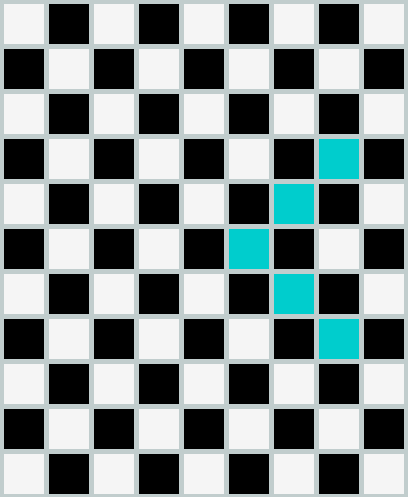
\includegraphics[scale=0.35]{immagini/goodCC}}
	\hspace{5mm}
	{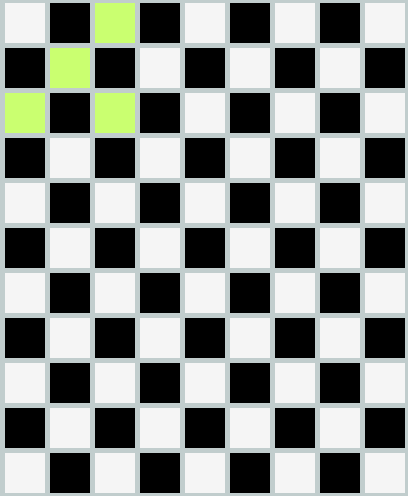
\includegraphics[scale=0.35]{immagini/badCC}}
	\caption{La figura a sinistra rappresente un valore consistente per la forma a "V", mentre la figura a destra uno non valido per la figura a "T" in quanto si crea una componente connessa di una sola cella}
	\label{fig:badCC}
\end{figure}

\subsection{Tipi di solver}
La libreria \textit{python-constraint} che abbiamo utilizzato per risolvere il problema sotto forma di CSP, mette a disposizione tre diversi solver, che utilizzano algoritmi ed euristiche differenti per ottenere una soluzione. \\
Inoltre abbiamo incluso e modificato il codice della libreria all'interno del nostro progetto per poter visualizzare nella griglia grafica ogni passo di computazione dei vari solver e aggiungere alcune migliorie esposte in \ref{migliorie}.
\subsubsection{Backtracking}
Questo solver ad ogni passo di computazione seleziona la prossima variabile a cui assegnare un valore attraverso l'euristica di grado, cioè per ogni variabile conta il numero di vincoli in cui è coinvolta, selezionando quella più vincolata. Qualora questa euristica evidenzi più di una variabile, a queste viene applicata l'euristica Minimum Remaining Values (MRV), che seleziona la variabile con il minor numero di valori nel dominio.\\
Una volta scelta la variabile le viene assegnato un valore consistente con l'assegnamento parziale, se esiste, eliminando dai domini delle altre variabili, attraverso un \textit{forward checking}, i valori non più consistenti con il nuovo assegnamento. Se non esiste un valore consistente nel dominio della variabile, si ritorna all'ultima variabile assegnata, cambiandone il valore. \\
Quando tutte le variabili hanno un valore nell'assegnamento, esso viene ritornato come soluzione del problema.
\subsubsection{Backtracking ricorsivo}
Utilizza lo stesso algoritmo esposto nel paragrafo precedente, solamente che viene implementato in modo ricorsivo.
\subsubsection{MinConflict}
Questo solver utilizza un algoritmo di ricera locale cioè, partendo da un assegnamento completo delle varibili, cerca di ottenere una soluzione al problema modificando ad ogni passo il valore di una variabile, facendo in modo che violi il minor numero di vincoli del problema. \\
Questi tipi di algoritmi non considerano il percorso per raggiungere una soluzione, ma danno importanza solamente alla configurazione finale. Inoltre utilizzando un unico stato corrente, possono portare alla soluzione utilizzando poca memoria, e spesso si rivelano più efficienti nel caso di un grande spazio degli stati, rispetto ad altri algoritmi.\\

\begin{figure}[h]
	\centering
	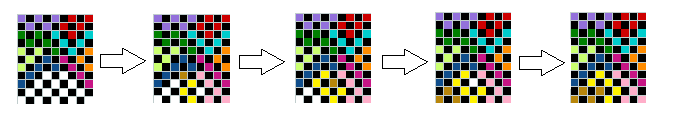
\includegraphics[scale=0.75]{immagini/mc}
	\caption{Funzionamento del solver MinConflict (da notare che alcune forme sono sovrapposte e quindi non del tutto visibili)}
	\label{fig:mc}
\end{figure}


\newpage
\section{Nostri miglioramenti}
\label{migliorie}
Una volta implementati gli algoritmi appena visti, abbiamo pensato a dei modi per poter miglorare la loro efficienza rispetto al nostro gioco. \\

\subsection{Connected Component Check}
Per quanto rigurda DFS, Backtracking e Backtracking ricorsivo abbiamo aggiunto un particolare controllo, se voluto dall'utente attraverso uno specifico input, chiamato \textbf{Connected Component Check}.
Durante l'esecuzione dei vari algoritmi, nel momento in cui viene deciso un valore per la prossima variabile da assegnare, insieme all'assegnamento parziale ottenuto fino a quel momento, viene fatto un controllo sulla dimensione della minima componente connessa rimanente nella griglia. \\
Se essa ha una dimensione minore della più piccola forma ancora da inserire, viene scartato il nuovo valore che si stava assegnando alla variabile e ne viene analizzato un altro. 

\begin{figure}[h]
	\centering
	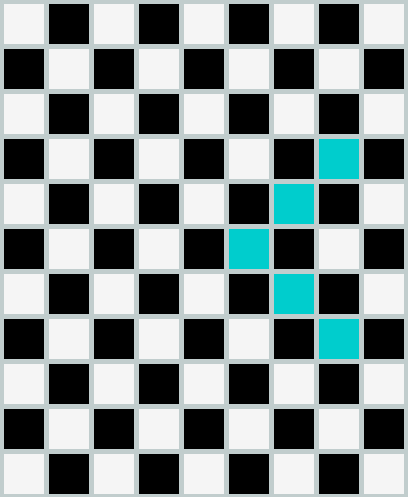
\includegraphics[scale=0.25]{immagini/goodCC}
	\caption{Assegnamento consistente per la variabile "V"}
	\label{fig:CCC}
\end{figure}

\begin{figure}[h]
	\centering
	{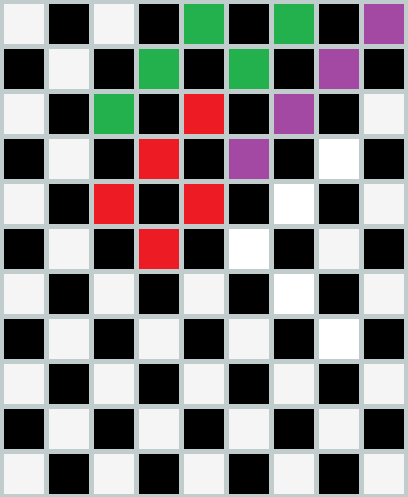
\includegraphics[scale=0.35]{immagini/esCC}}
	\hspace{5mm}
	{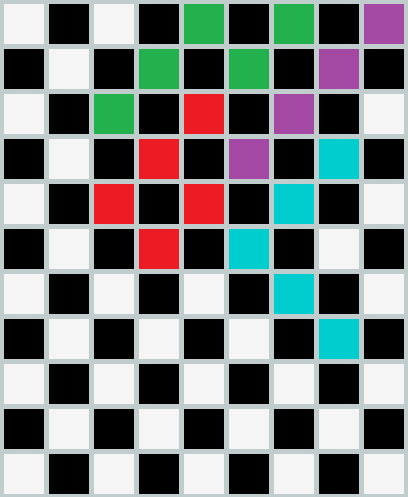
\includegraphics[scale=0.35]{immagini/esCC_no}}
	\caption{La stessa posizione della figura \ref{fig:CCC} per la variabile "V" non è consistente con l'assegnamento parziale, e l'algoritmo che fa uso di Connected Component Check è in grado di rilevarlo}
	\label{fig:badCCC}
\end{figure}

\subsection{Random Restart}
Abbiamo notato come il solver MinConflict nelle istanze complesse del problema non raggiunga un assegnamento completo e consistente, ossia una soluzione. Questo è dovuto dal fatto che può capitare di raggiungere stati dove ogni possibile successiva azione non diminuisce il numero di vincoli violati. Nel caso in cui l'algoritmo arrivi in uno di questi stati, chiamati minimi locali, non è più in grado di raggiungere una soluzione del problema, in quanto inizia una serie di assegnamenti ciclici che lo porteranno sempre allo stesso minimo locale, terminando dopo un numero fissato di iterazioni in un assegnamento non consistente.\\
Per ovviare a questo problema l'utente ha la possibilità, tramite uno specifico input nella definizione del problema, di utilizzare la tecnica chiamata Random Restart. Essa consiste nel riavviare l'algoritmo qualora termini con un assegnamento non consistente, finchè non ritorna una soluzione valida per il problema. Questa tecnica rende MinConflict completo, in quanto ci assicura di ottenere sempre un assegnamento completo e consistente, dopo un certo numero di riavvii.\\



 